\section{数据收集与分析}
\subsection{需要数据与预估收集方式}
\begin{itemize}
    \item [\textbf{$\bullet $}] 确定校园满足充电桩建设的地点地点位置级数量、 校方目前在其中地建设了充电桩的地点位置级数量、所有充电桩建设地点拥有充电口总数$\implies $\textit{自行在校园内排查}
    \item [\textbf{$\bullet $}] 校内拥有需充电设备的师生最常去的几个地点地区$\implies $\textit{问卷调查}
    \item  [\textbf{$\bullet $}]以及点与点间的距离进行统计$\implies $\textit{自行在校园内排查}
    \item [\textbf{$\bullet $}]师生的充电偏好(充电时间/充电时长/周充电频率等)$\implies $\textit{问卷调查}
\end{itemize}
\subsection{数据呈现}
\begin{figure}[H]
	\centering
	\subcaptionbox{可行的30处充电桩建设点}{
		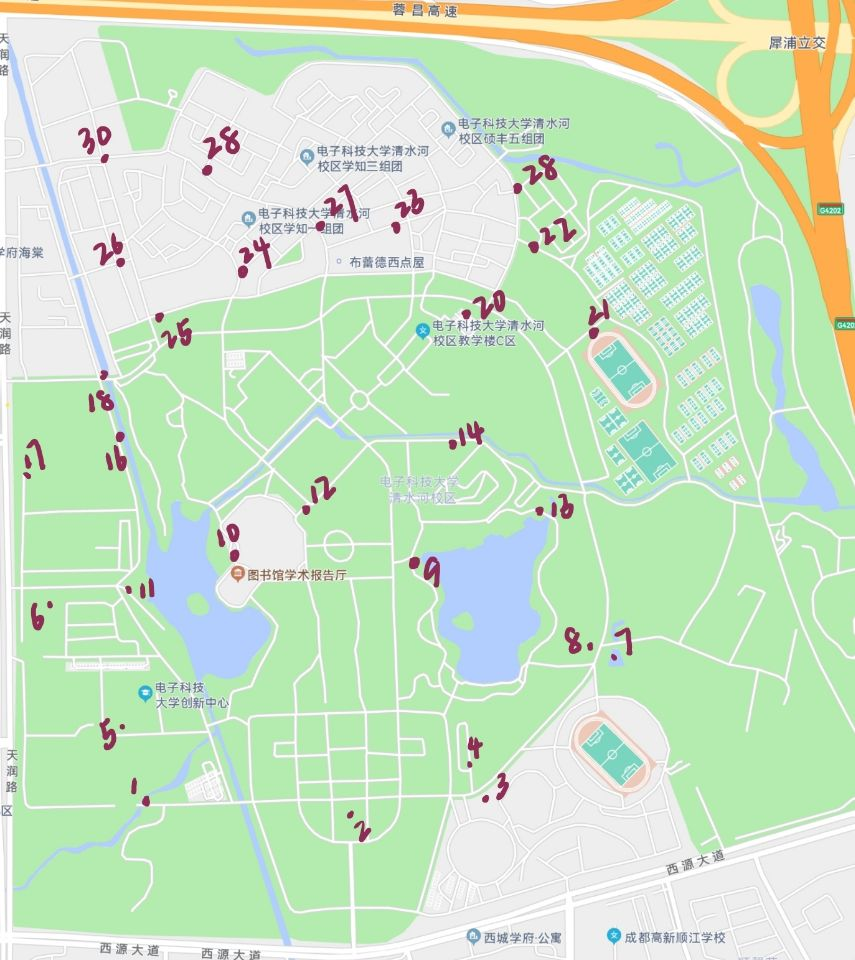
\includegraphics[width=5.5cm]{pic2.jpg}		
	}
	%\hfill % 是为了让多幅图在一行均匀分布(不加的效果是都挤在中间)
	\subcaptionbox{研究生通常活动区域}{
		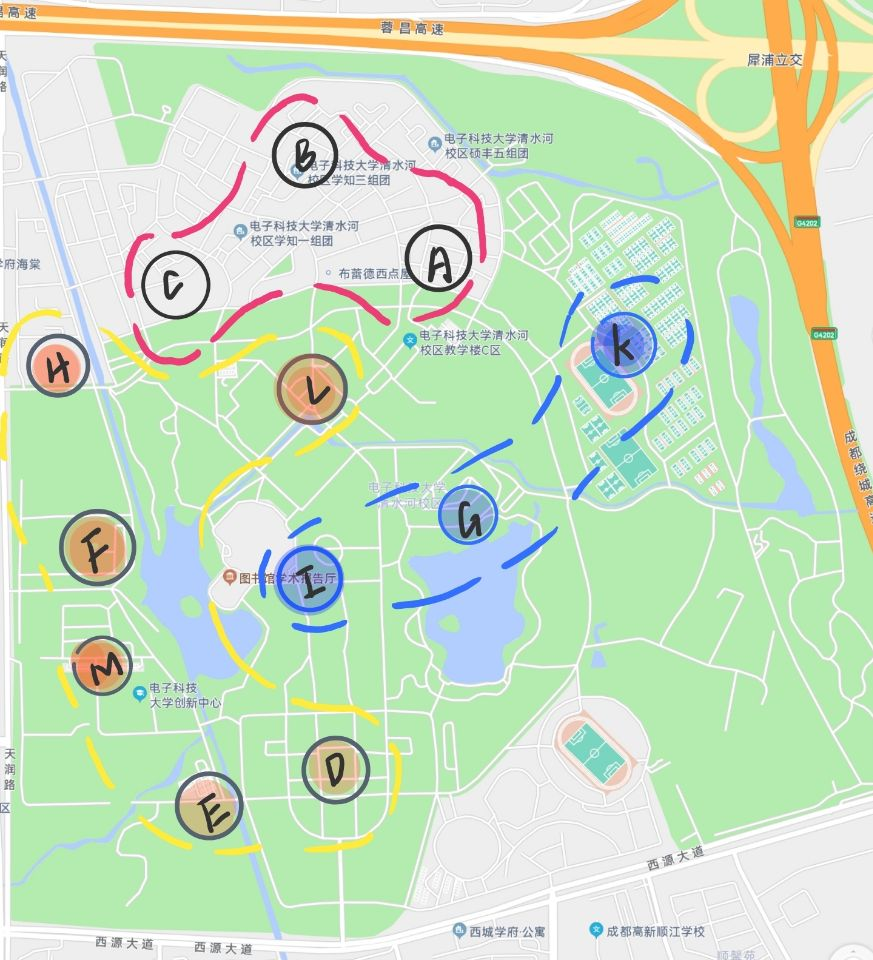
\includegraphics[width=5.5cm]{pic3.jpg}	
	}
	
	\label{functionrelationship}
\end{figure}

\begin{table}[H]\small
	\centering
	\caption{通常活动区域\textit{常驻地}与充电桩\textit{目的地}间距离}
	%\label{频率型、强度型和相对比型指标}也可以用这个
	\begin{tabular}{c|p{0.60cm}<{\centering}|p{0.6cm}<{\centering}|p{0.6cm}<{\centering}|p{0.6cm}<{\centering}|p{0.6cm}<{\centering}|p{0.6cm}<{\centering}|p{0.6cm}<{\centering}|p{0.6cm}<{\centering}|p{0.6cm}<{\centering}|p{0.6cm}<{\centering}|p{0.6cm}<{\centering}|p{0.54cm}<{\centering}}
		\toprule[2pt]  %添加表格头部粗线
		\diagbox{\footnotesize {目的地$j$}}{\footnotesize {距离($m$)}}{\footnotesize {常驻地$i$}} &  A & B & C & D & E & F & M & L & H & I & G & K \\
		\midrule[1.75pt]  %添加表格中横线
		1 & 1900 & 1900 & 1551 & 317 & 15 & 518 & 680 & 1420 & 1304 & 797 & 751 & 2456 \\ 
        2 & 1474 & 1474 & 1474 & 0 & 233 & 714 & 363 & 1185 & 1227 & 564 & 564 & 2030 \\ 
        3 & 1518 & 1518 & 1518 & 252 & 485 & 966 & 615 & 1418 & 1271 & 797 & 751 & 2074 \\ 
        4 & 1557 & 1557 & 1557 & 321 & 554 & 1035 & 684 & 1463 & 1310 & 807 & 838 & 2113 \\ 
        5 & 1780 & 1780 & 1431 & 456 & 223 & 473 & 102 & 1566 & 1184 & 926 & 796 & 2336 \\ 
        6 & 1379 & 1379 & 1030 & 728 & 495 & 239 & 31 & 1168 & 783 & 1136 & 986 & 1935 \\ 
        7 & 1200 & 1300 & 1300 & 652 & 885 & 1366 & 1074 & 1179 & 1053 & 878 & 541 & 1756 \\ 
        8 & 900 & 991 & 991 & 925 & 1158 & 1639 & 1347 & 882 & 744 & 538 & 201 & 1456 \\ 
        9 & 906 & 906 & 906 & 564 & 797 & 1278 & 986 & 1155 & 659 & 121 & 21 & 1462 \\ 
        10 & 914 & 914 & 856 & 702 & 935 & 1416 & 1124 & 439 & 609 & 31 & 210 & 1470 \\ 
        11 & 1300 & 1300 & 951 & 714 & 481 & 11 & 1136 & 762 & 704 & 1265 & 1195 & 1856 \\ 
        12 & 838 & 838 & 489 & 798 & 1031 & 1512 & 1220 & 390 & 242 & 82 & 121 & 1394 \\ 
        13 & 1000 & 1000 & 1000 & 1000 & 1233 & 1714 & 1422 & 1034 & 753 & 426 & 89 & 1556 \\ 
        14 & 848 & 848 & 848 & 1240 & 1473 & 1954 & 1662 & 882 & 601 & 426 & 89 & 1404 \\ 
        15 & 658 & 658 & 358 & 867 & 1100 & 1581 & 1289 & 178 & 111 & 212 & 242 & 1214 \\ 
        16 & 1000 & 1000 & 700 & 966 & 733 & 100 & 329 & 452 & 453 & 938 & 1326 & 1556 \\ 
        17 & 1100 & 1100 & 800 & 1103 & 870 & 100 & 379 & 452 & 553 & 938 & 1326 & 1656 \\ 
        18 & 868 & 868 & 519 & 1115 & 882 & 360 & 510 & 889 & 272 & 1375 & 1230 & 1424 \\ 
        19 & 626 & 626 & 500 & 1185 & 1418 & 882 & 1607 & 32 & 253 & 439 & 793 & 1182 \\ 
        20 & 306 & 584 & 584 & 1406 & 1639 & 1539 & 1828 & 149 & 337 & 635 & 738 & 862 \\ 
        21 & 454 & 875 & 875 & 1791 & 2024 & 1420 & 2213 & 534 & 628 & 1020 & 991 & 0 \\ 
        22 & 290 & 654 & 654 & 1621 & 1854 & 1340 & 2043 & 364 & 897 & 850 & 1082 & 231 \\ 
        23 & 200 & 350 & 350 & 1385 & 1618 & 1104 & 1807 & 128 & 593 & 614 & 707 & 756 \\ 
        24 & 572 & 572 & 133 & 1364 & 1131 & 715 & 844 & 107 & 815 & 593 & 891 & 1128 \\ 
        25 & 758 & 758 & 319 & 1478 & 1245 & 615 & 744 & 221 & 1001 & 707 & 991 & 1314 \\ 
        26 & 817 & 726 & 340 & 1572 & 1339 & 654 & 783 & 315 & 969 & 801 & 1080 & 1373 \\ 
        27 & 520 & 258 & 258 & 1223 & 1456 & 1310 & 1439 & 152 & 501 & 638 & 707 & 1076 \\ 
        28 & 329 & 469 & 719 & 1791 & 2024 & 1327 & 2213 & 534 & 712 & 1020 & 1201 & 389 \\ 
        29 & 770 & 129 & 129 & 1538 & 1771 & 1239 & 1360 & 281 & 372 & 767 & 919 & 1326 \\ 
        30 & 953 & 567 & 149 & 1730 & 1497 & 897 & 1018 & 473 & 810 & 959 & 1102 & 1509 \\ 
		\bottomrule[2pt] %添加表格底部粗线
	\end{tabular}
\end{table}
我们将学生常去的地区\textit{常驻地},做出三种分类:宿舍区(ABC),学习/教研室区(DEFMLH),休闲/其他常去区(IGK)。\\
\indent 以下表格根据问卷结果与实际学院人数、对应教研室位置做出统计:
\begin{table}[H]
    \centering
	\caption{收集问卷结果:学生常去区域的时间分配$S_{k}$}
    %\label{频率型、强度型和相对比型指标}也可以用这个
    \begin{tabular}{c|p{2cm}<{\centering}|p{3cm}<{\centering}|p{3cm}<{\centering}}
        \toprule  %添加表格头部粗线
        \diagbox{常去情况}{区域} & 宿舍区(ABC) & 学习区(DEFMLH)& 其他休闲区(IGK)  \\
        \midrule  %添加表格中横线
        时间分配 & 30\% & 60\% & 10\%\\
        
        \bottomrule %添加表格底部粗线
    \end{tabular}
\end{table}

\begin{table}[H]
    \centering
	\caption{问卷数据统计结果:宿舍区}
    \begin{tabular}{c|p{3cm}<{\centering}|p{3cm}<{\centering}|p{3cm}<{\centering}}
        \toprule  %添加表格头部粗线
        \diagbox{情况}{常驻地} & A & B& C \\
        \midrule  %添加表格中横线
        学生比例分配 & 33.33\% & 33.33\% & 33.33\%\\
        \bottomrule %添加表格底部粗线
    \end{tabular}
\end{table}
\begin{table}[H]
    \centering
	\caption{实际学院人数数据计算结果:学习区}
    \begin{tabular}{c|p{1.7cm}<{\centering}|p{1.7cm}<{\centering}|p{1.7cm}<{\centering}|p{1.7cm}<{\centering}|p{1.7cm}<{\centering}|p{1.7cm}<{\centering}}
        \toprule  %添加表格头部粗线
        \diagbox{情况}{常驻地} & D & E& F&M&L&H \\
        \midrule  %添加表格中横线
        学生比例分配 & 18.93\%&	11.27\%&	29.06\%&	12.74\%&	18.12\%&	9.87\%\\

        \bottomrule %添加表格底部粗线
    \end{tabular}
\end{table}
\begin{table}[H]
    \centering
	\caption{问卷数据统计结果:其他休闲区}
    \begin{tabular}{c|p{2cm}<{\centering}|p{3cm}<{\centering}|p{3cm}<{\centering}}
        \toprule  %添加表格头部粗线
        \diagbox{情况}{常驻地} & I & G& K \\
        \midrule  %添加表格中横线
        学生比例分配 & 50\% & 20\% & 30\%\\
        \bottomrule %添加表格底部粗线
    \end{tabular}
\end{table}